\documentclass[a4paper,12pt]{article}
\usepackage{hyperref}
\usepackage{times}
\usepackage{comment}
\usepackage{titlesec}
\usepackage[pdftex]{graphicx}

\usepackage{geometry}
\geometry{lmargin=1.5cm,rmargin=1.5cm,height=25cm}
\renewcommand{\thesubsection}{\Roman{subsection}}

\begin{document}
\title{INTERPRETING ST. LAWRENCE}
\author{Joanna Lace}
\date{}
\maketitle


The centenary year of St.~Lawrence seems an appropriate time to
consider anew some aspects of a painting of the saint now in the
Widnacourt Museum\footnote{Donated to the museum by the Fabri family
  of Vittoriosa.}. A new series of photographs has literally thrown
new light on this work, bringing out its true colouring and revealing
the landscape background--features that can now be enjoyed by those of
us not readily able to make a personal visit\footnote{I am indebted to
  Mr. Peter Bartolo Parnis for these professional
  photographs.}. [Fig.1]
\begin{center}
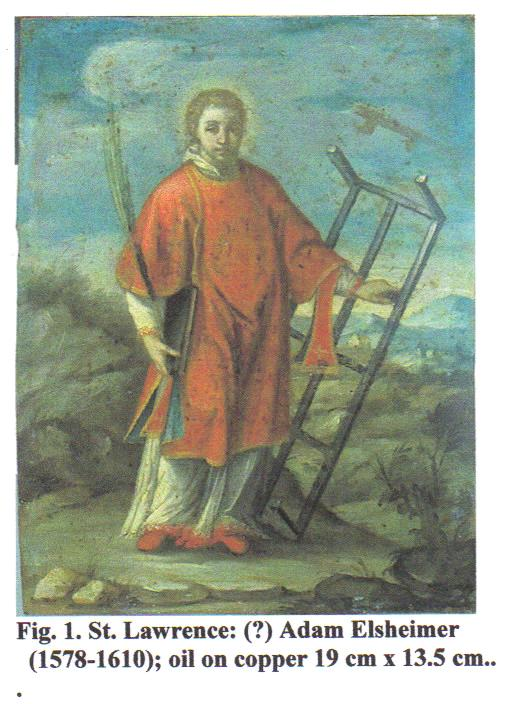
\includegraphics[width=10cm]{fig1.jpg}
\end{center}

It has been suggested that it was painted by Adam Elsheimer, an artist
whose true import and influence has recently been recognised through a
superb retrospective exhibition ``Devil in the Detail: the paintings
of Adam Elsheimer 1578--1610'', held during 2006 at Frankfurt,
Edinburgh and then London.  Although it must be said that neither the
devil nor the detail of Elsheimer's paintings are present in the
St.Lawrence work, the publication that accompanied this exhibition is
a mine of up-to-date information, not only on Elsheimer himself--his
life, his art and its influence--but includes helpful references to
the art of his close artistic circle during the ten years he lived in
Rome until his death there at the early age of 32, including their
mutual borrowings and their cooperative ventures\footnote{See
  R. Klessmann, \textit{Adam Elsheimer 1578--1610}, Trustees of the
  National Galleries of Scotland in association with Dulwich Picture
  Gallery (paperback), 2006, and Paul Holberton Publishing (hardback),
  2006; published to accompany the exhibition ``\textit{Devil in the
    Detail: the paintings of Adam Elsheimer 1578--1610}''. It should be
  pointed out that the German edition includes full entries on
  Elsheimer’s contemporaries in Rome, and an expanded discussion of
  the works of some fellow artists, concluding that they studied
  together rather than actually worked with him or shared a workshop.
}. It will certainly be the starting point for future in-depth
investigations.

Meanwhile some findings of a less technical nature help to explain the
context and then some of the features the Widnacourt St.~Lawrence.  As
a starting point, brief notes on the practice of painting on copper
provide a general background, in that the painting is an example of
what was to become the preferred method for the widespread production
of small decorative objects over a period of about two hundred years.
The subject has also recently been the subject of wide-ranging
research, so that we know more than ever before about copper
production, marketing, its popularity among artists, and the various
techniques they used\footnote{See \textit{Copper as Canvas, Two
    Centuries of Masterpiece Paintings on Copper 1575--1775}, Phoenix
  Art Museum and Oxford University Press, 1999; accompanying the
  exhibition organised by the Phoenix Art Museum, held in 1999 at
  Phoenix Art Museum, The Nelson Atkins Museum of Art, and the Royal
  Cabinet of Paintings, Mauritshuis, The Hague.  }. Following this,
details revealed by the photographs point to the comparatively
traditional nature of the landscape, and from this, something about
the artist concerned.

It is very probable that painting in oils on copper originated in
Italy, and isolated examples are known from the first half of the
sixteenth century.  The smooth surface of prepared copper lends itself
to painting on an almost incredibly small scale.  Later in the
century, where the chosen subject seemed appropriate, artists learnt
to fill the whole surface of a cabinet picture or other small object
with a design of tiny figures--sometimes dozens--and sometimes using
an eye-glass.  General admiration at the sheer skill involved led to
these creations being considered rare and precious, `objets de vertu',
much sought after by collectors, and still in evidence today in princely
collections.

In the 1590s the Flemish artist Paul Bril, one of a number of northern
artists drawn to Rome, began to work on copper.  The advantages that
made it so suitable for paintings on a small scale--the meticulous
details of colour and texture, and the wonderful effects of light and
shade achievable on its exceptionally smooth and non-absorbent
surface--Bril used to create splendidly naturalistic landscape
backgrounds for his paintings.

Bril's friend Elsheimer arrived in Rome in 1600, and was one of the
first of a group of artists in Rome to take up the practice with
enthusiasm. They were almost exclusively recent arrivals from northern
Europe, known collectively as the \textit{compagnen}.  All expressed
true amazement at the new naturalism, luminosity, and minute detail of
Elsheimer's landscapes: they brought him instant fame, and marked a
turning point not only for him but for the seventeenth century as a
whole, becoming a stage in the gradual progression towards the
painting of landscape for its own sake.

By the turn of the century the use of copper was the northerners'
choice not only for landscapes but still lifes, portraits,
mythological and devotional subjects, as well as for reduced copies of
easel paintings and altarpieces.  Copies were usually made by
anonymous copyists, and there are cases of multiple versions of a
single composition.  It was also in Rome that paintings on copper
first became a collaborative exercise, perhaps because painting itself
was tending to separate into different genres, some artists being
considered adept at figures, and others chosen for their artistry with
landscape.

Apart from the advantage of needing a less elaborate preparation than
traditional supports, a copper support was durable, easy to transport,
and, as recent studies now indicate, no more expensive.  Small
paintings that could be held in the hand became extremely popular as
gifts for personal use, either of a devotional nature--as papal gifts,
for young girls upon taking the veil--or with a secular theme for
young brides and others.  They were also let into furniture, again
both in liturgical and devotional contexts such as shrines and
portable altars, and in secular interiors as embellishment on the
fronts of drawers, shutters, and doors.

A series of small panels by Elsheimer dated to c.1605 is believed to
have been intended for use in this way for the decoration of a
valuable cabinet.  Each portrays, within a landscape, a single
standing figure or a pair of figures from the Old or New Testament.
Eight of these panels are now in Petworth, England, and another of the
same series, now in Montpelier, France, portrays St.~Lawrence.[Fig.2]
\begin{center}
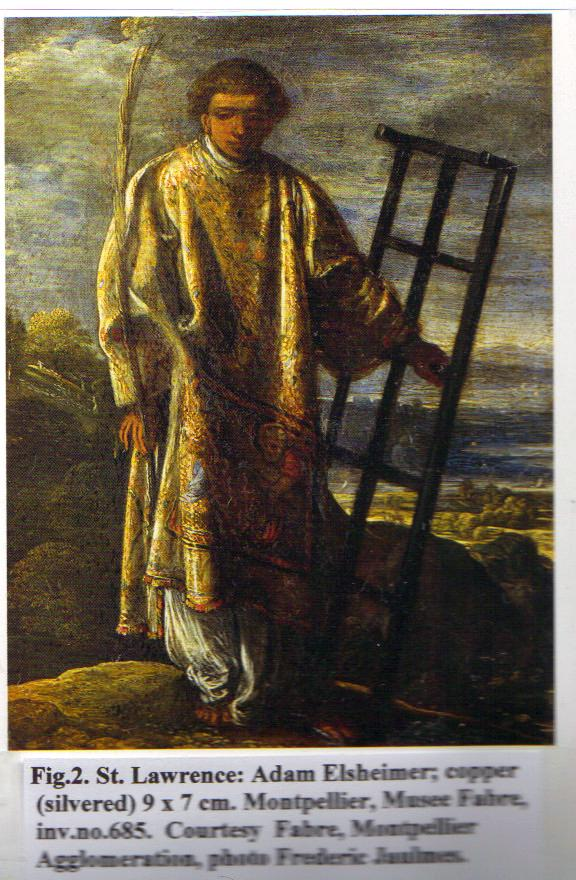
\includegraphics[width=10cm]{fig2.jpg}
\end{center}
In the positioning of the saint's emblems, in particular the
grid-iron, held out prominently at arm's length and shoulder-high, it
is similar to our Widnacourt version, and this has suggested that the
latter may also have been painted by Elsheimer\footnote{See
  ed. J.Azzopardi, \textit{St.Paul's Grotto, Church and Museum at
    Rabat, Malta}, Malta 1990, p.394.}. However, it is the differences
between the two paintings that may well hold the answer to the
Widnacourt artist's identity, particularly as we are now told that
there is no written evidence for copies by Elsheimer himself of his
own paintings.  This fact is borne out by chroniclers' mention of his
``slow method'', his ``unproductiveness'', and by Rubens' reference to
his ``accidia'' (sloth), and the considerable number of his unfinished
works.  In fact the only copies of the panels that we have secure
knowledge of so far are by the Utrecht artist Cornelius van
Poelenburgh (1586/7--1667), and are now in Florence: they are true
copies of the Elsheimers, exact in every detail.  At the same time, in
the particular workshop environment of the \textit{compagnen}, where
quite often features of a `copy' differed from the original,
noticeable differences with respect to Elsheimer's St.~Lawrence should
point the way forward to an examination of the paintings of his artist
friends, and their collaborative works.

To begin with differences of figure style: unless saints are part of a
narrative, they are habitually shown accompanied by their attributes.
Elsheimer's figure holds his grid-iron firmly, standing straight but
with head slightly forward and eyes half closed--a meditative
pose.[Fig.3] The Wignacourt artist presents the young saint with a
softly glowing halo, in arrested movement, feet placed apart, as if
pausing momentarily to look directly at the viewer; and a certain
elegance is discernible in the positioning of the hands and the sway
of his lower garment.
\begin{center}
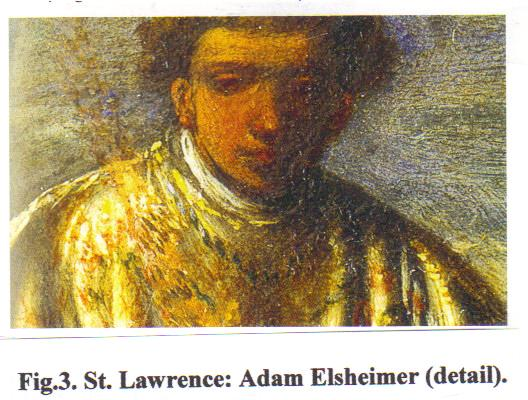
\includegraphics[width=12cm]{fig3.jpg}
\end{center}

Turning to the landscape, as part of a figural painting this can also
be a guide to an artist's general perception of the overall scene. Its
inclusion behind the representation of a holy figure had become
customary, whether or not it were factually relevant--the present
example of St.~Lawrence, a young deacon who had lived in the crowded
city of Rome amongst the poor, being a case in point.  Already with
D\"urer a century earlier, its inclusion was seen as an asset, lending a
contemplative mood to the work, as in numerous paintings of the Virgin
and Child.  On occasion a patron would stipulate a landscape
background when commissioning a devotional painting.

However, Elsheimer's landscape has been given a new role, for which he
has devised a personal format.  It is no longer a background `extra',
but has become the living habitat of the figure, in a form integral to
the message being conveyed.  He discards the traditional `coulisse'
method seen in his earlier paintings, where strategically-placed
figures, paths, trees, all decreased gradually in size towards the
horizon, which was itself often hidden behind mountains or forests
rising high in the distance\footnote{For an example of earlier
  Elsheimer landscapes, see the side panels of his altarpiece `The
  True Cross' (or `The Frankfurt Tabernacle'), now in Frankfurt, dated
  1603--05.}. Instead, he opens up a panorama of unprecedented depth by
a highly original deployment of light, which glances sporadically on
minute features of the land and of country life – such as a tiny
upland, a stretch of water, a lone rider, animals, birds.[Fig.4]
\begin{center}
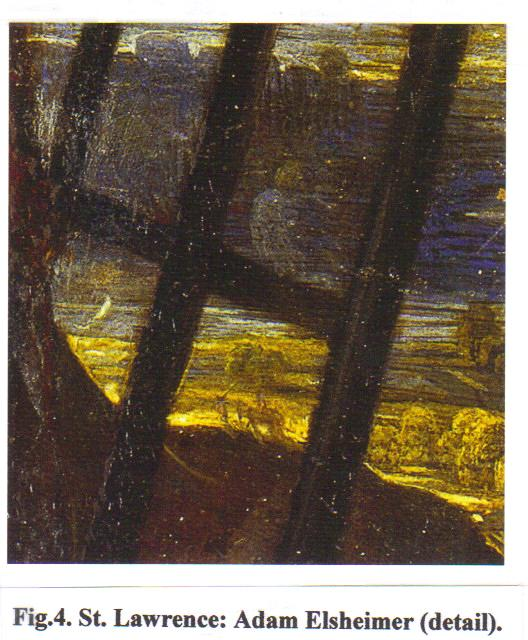
\includegraphics[width=10cm]{fig4.jpg}
\end{center}
Against this the figure of St.~Lawrence gains in monumentality from a
low viewpoint and its position right to the front of the picture
plane, extending almost to its upper edge; it is well lit, and
portrayed in light colours. The ground he stands on appears to drop
abruptly behind him to the vastness below--an inhabited vastness, and
one that is essentially portrayed as part of the saint's own living
environment.

The Wignacourt figure of St.~Lawrence cannot be said to appear
similarly incorporated in his surroundings, which are of a different
order, and like the painting as a whole have a different appeal.  The
landscape colours follow an age-old tradition: blue for sky and the
far distance, and for the middle distance shades of dark brown, which
in this case continue down to the lower edge of the panel, creating a
rough terrain of boulders and low bushes.  In particular, the figure
of St.~Lawrence, notwithstanding the impression of movement noticed
earlier, is placed towards the centre of a level clearing: this is
marginally set back, its forward edge suggesting a platform on which
the saint is being presented to the viewer.[Fig.5] 
This way of
portraying a revered figure is also reminiscent of an ancient
tradition At the same time it must be said that even these traditional
features do not in themselves suggest an artist far from Elsheimer's
circle, given the large output of workshops and the tendency towards
cooperative practices\footnote{In this connection it has been noted
  that even a signed copy of an Elsheimer painting by Pieter Lastman,
  an ardent follower, is an adaptation, and by one who “probably did
  not understand [Elsheimer's] concerns”; see R. Klessmann,
  \textit{op.cit.} above, p.27.}.

It seems relevant in this year of St.~Lawrence to conclude by
recalling one of the legends concerning his martyrdom--one that will
0certainly have been known by the artists under review as well as
present readers.  As one of the deacons of the church appointed to
organise the provision of alms, Lawrence was ordered by the Prefect of
Rome, on pain of death, to hand over all `treasures', everything of
value, to the emperor for the upkeep of his armies.  He replied by
assembling from the streets of Rome many hundreds of the poor and
needy, and presented them, saying ``These are the treasures of the
church''.  This infuriated the Prefect, who promptly ordered his death
by slow roasting on a grid-iron.

We can never know the mind of an artist when he takes up his brush,
the viewer is thus at liberty to volunteer certain impressions.
Elsheimer's St.~Lawrence, for example, is a thinker, in line with the
ingenuity and resourcefulness under terrible pressure that is
expressed in the legend.  He is also the example, among all the
earth's created, living beings, of a monumental strength of purpose.

The Widnacourt St.~Lawrence has an ethereal quality: communicating a
youthful serenity despite recent horrors; not only undeterred by
inhospitable surroundings, he is already glorified, and turns to
address the viewer from another, eternal world.  A past commentator
has suggested that this work may be ``artistically superior'' to the
Elsheimer panel. Be that as it may, our comparisons have certainly
shown that St.~Lawrence has become, in the words of St. Paul
(referring to himself), ``all things to all men''.
\begin{center}
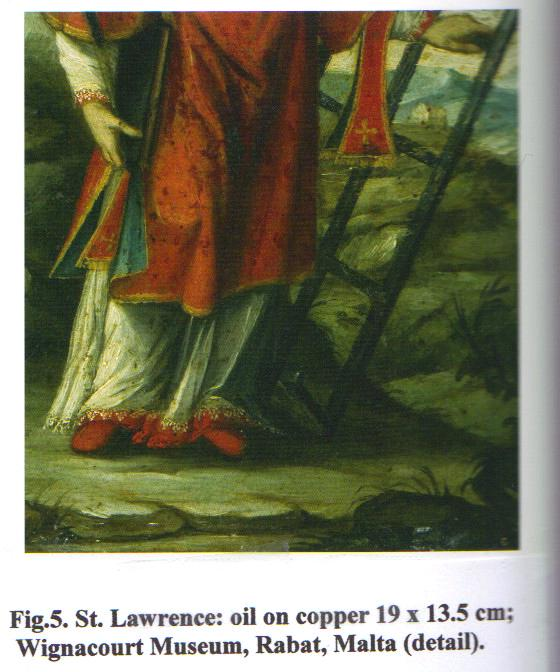
\includegraphics[width=10cm]{fig5.jpg}
\end{center}

\end{document}

